\begin{figure}[htbp]
\centering
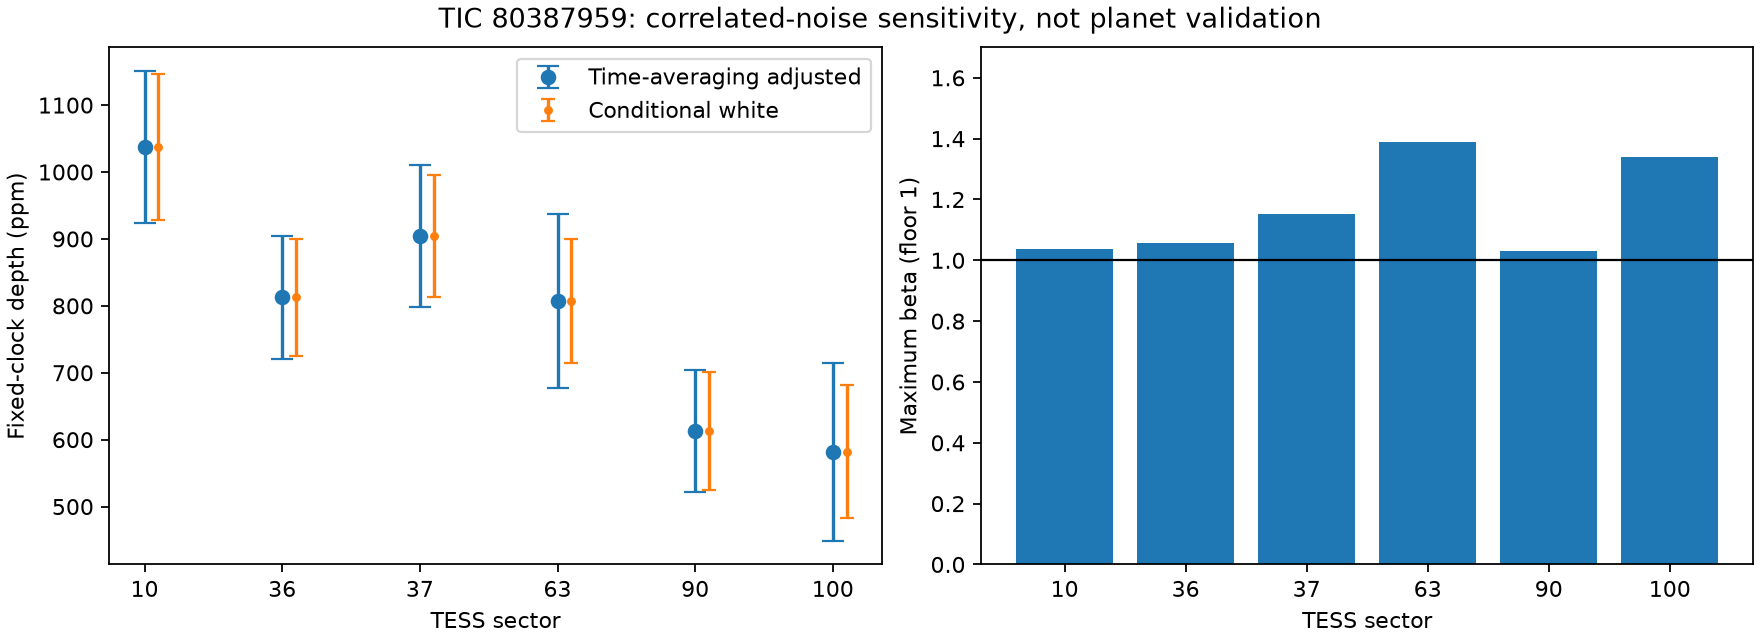
\includegraphics[width=\linewidth,height=0.72\textheight,keepaspectratio]{figures/803-noise.png}
\caption{TIC 80387959 time-averaging sensitivity. The six sector depths are retained while approximate error inflation and individual-event omissions reduce their apparent precision. The white-noise reference uses the same fitting design. Scalar inflation is not a complete correlated-noise model or a calibrated detection significance.}
\end{figure}
\begin{figure}[p]
\centering
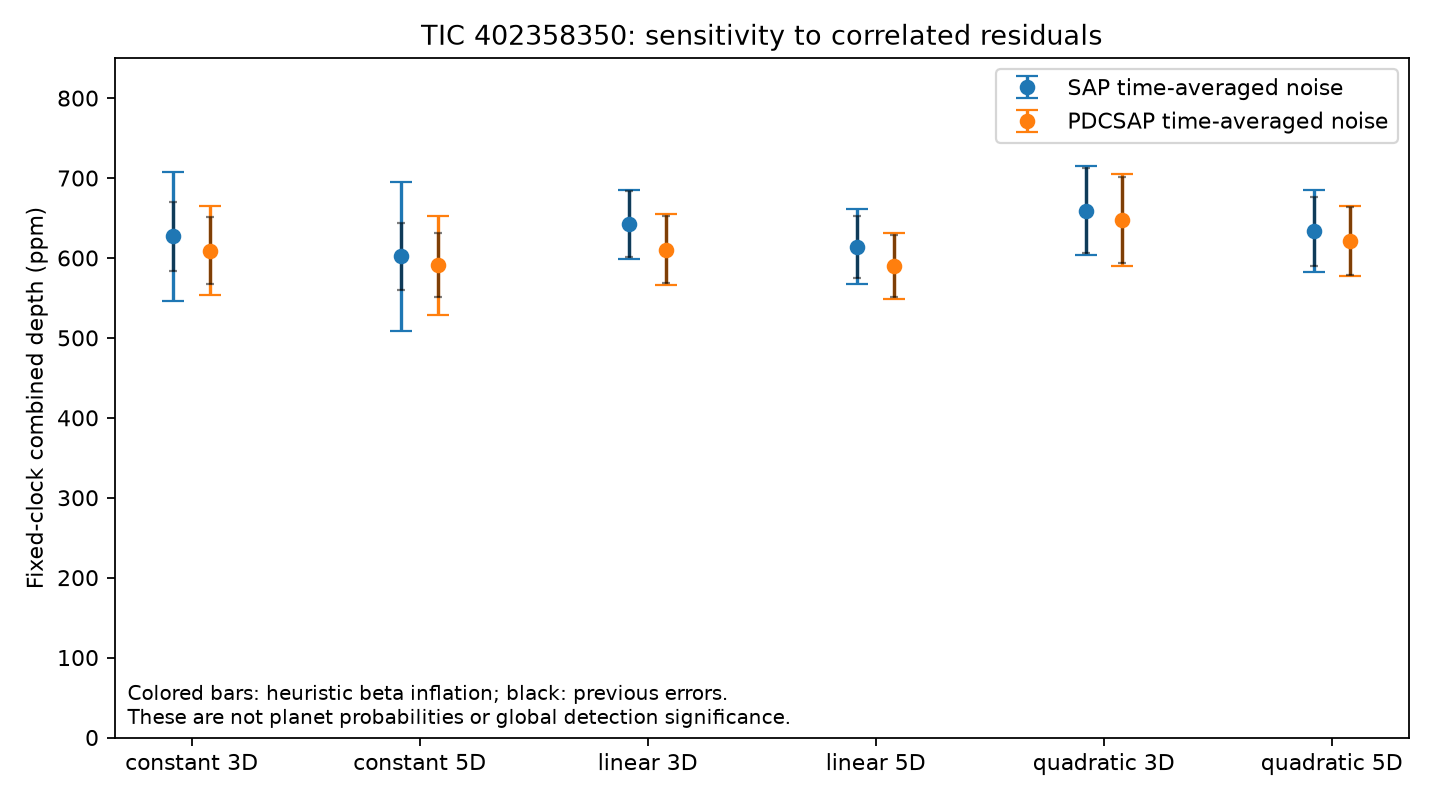
\includegraphics[width=\linewidth,height=0.72\textheight,keepaspectratio]{figures/402-noise.png}
\caption{TIC 402358350 noise sensitivity across the twelve SAP/PDC baseline methods. Missing or insufficiently populated time bins remain unavailable; the combined error range is 41--93 ppm. Reweighting the events is a separately labeled sensitivity test. These methods reuse the same eight events.}
\end{figure}
\begin{figure}[p]
\centering
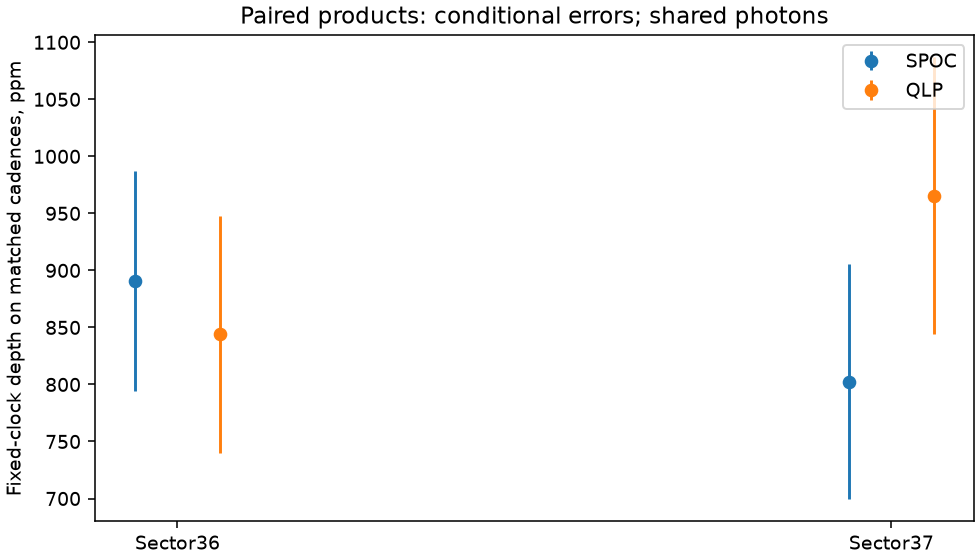
\includegraphics[width=\linewidth,height=0.72\textheight,keepaspectratio]{figures/803-paired.png}
\caption{TIC 80387959 paired SPOC/QLP reductions of the same sector-36/37 exposures. Differences depend on epoch and common-quality selection. They do not establish a universal QLP depth suppression or physical depth evolution.}
\end{figure}
\begin{figure}[p]
\centering
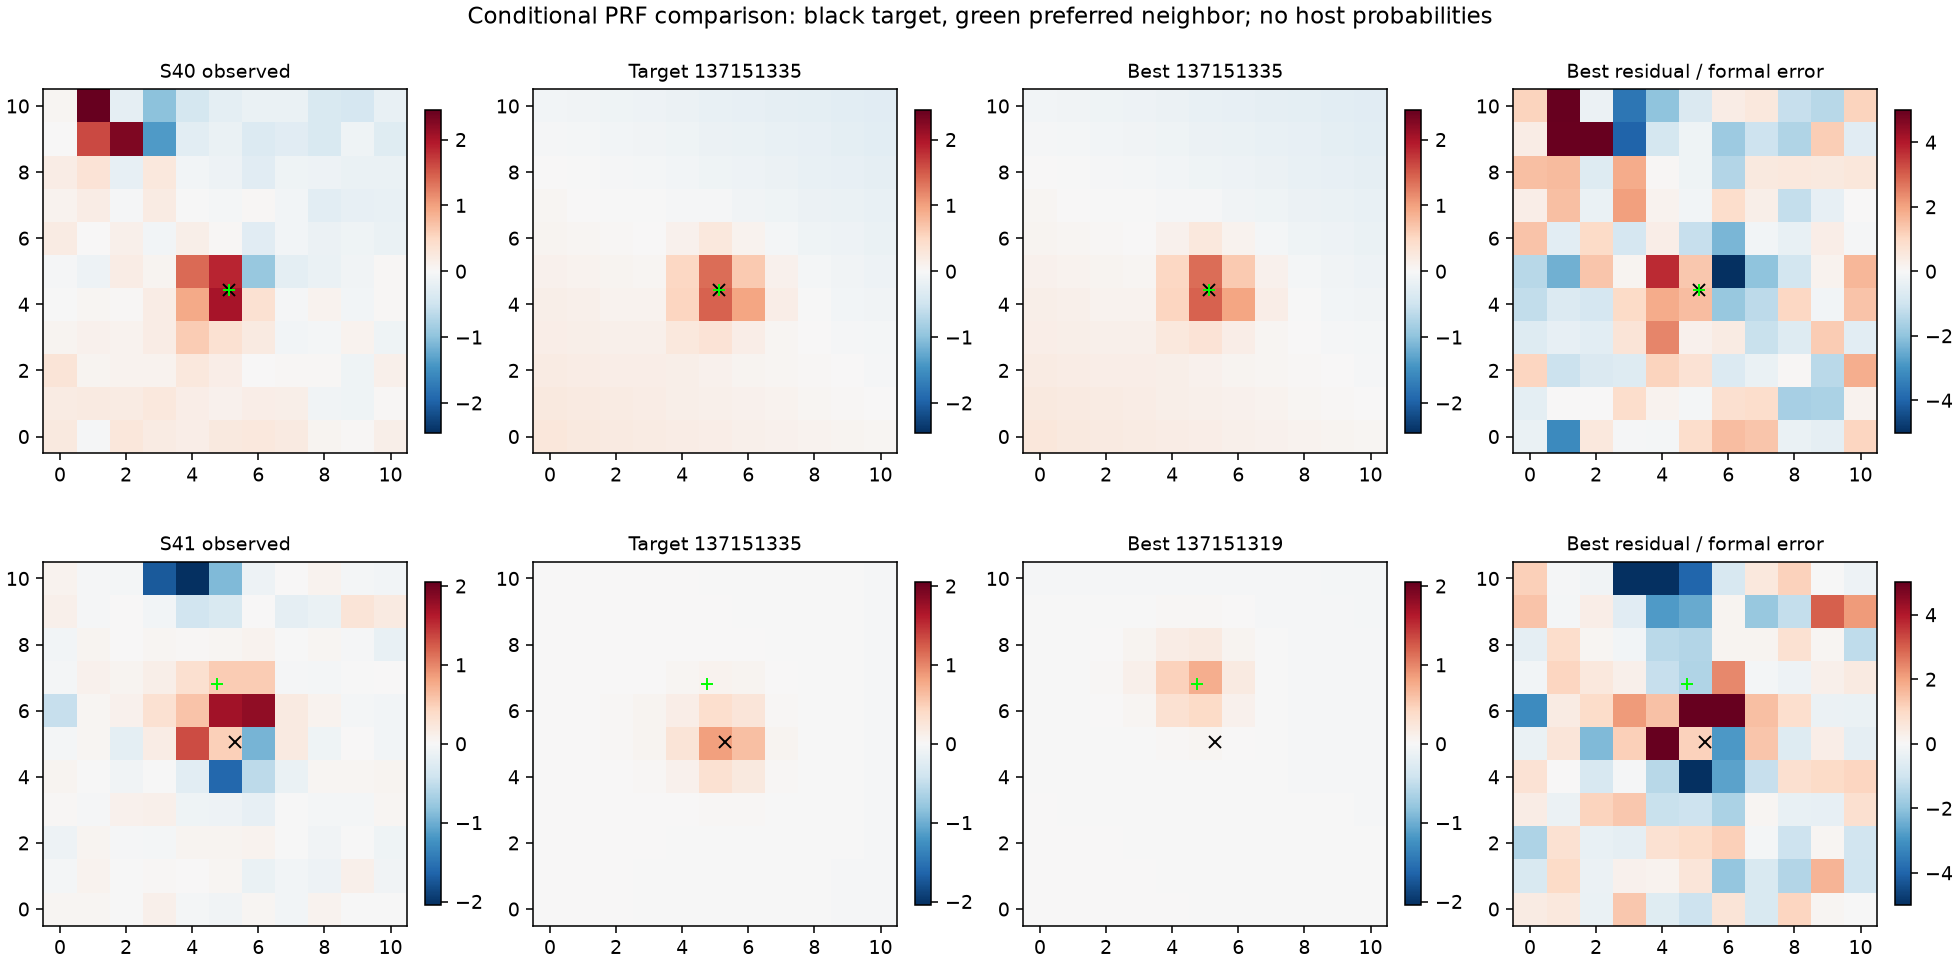
\includegraphics[width=\linewidth,height=0.72\textheight,keepaspectratio]{figures/host-control.png}
\caption{Known-host Kepler-93 b image control. The original template method prefers the correct target in sector 40 and a neighbor in sector 41 despite the established planetary signal. Structured residuals and wrong rankings undermine a probability interpretation of the same method on the candidates.}
\end{figure}
\begin{figure}[p]
\centering
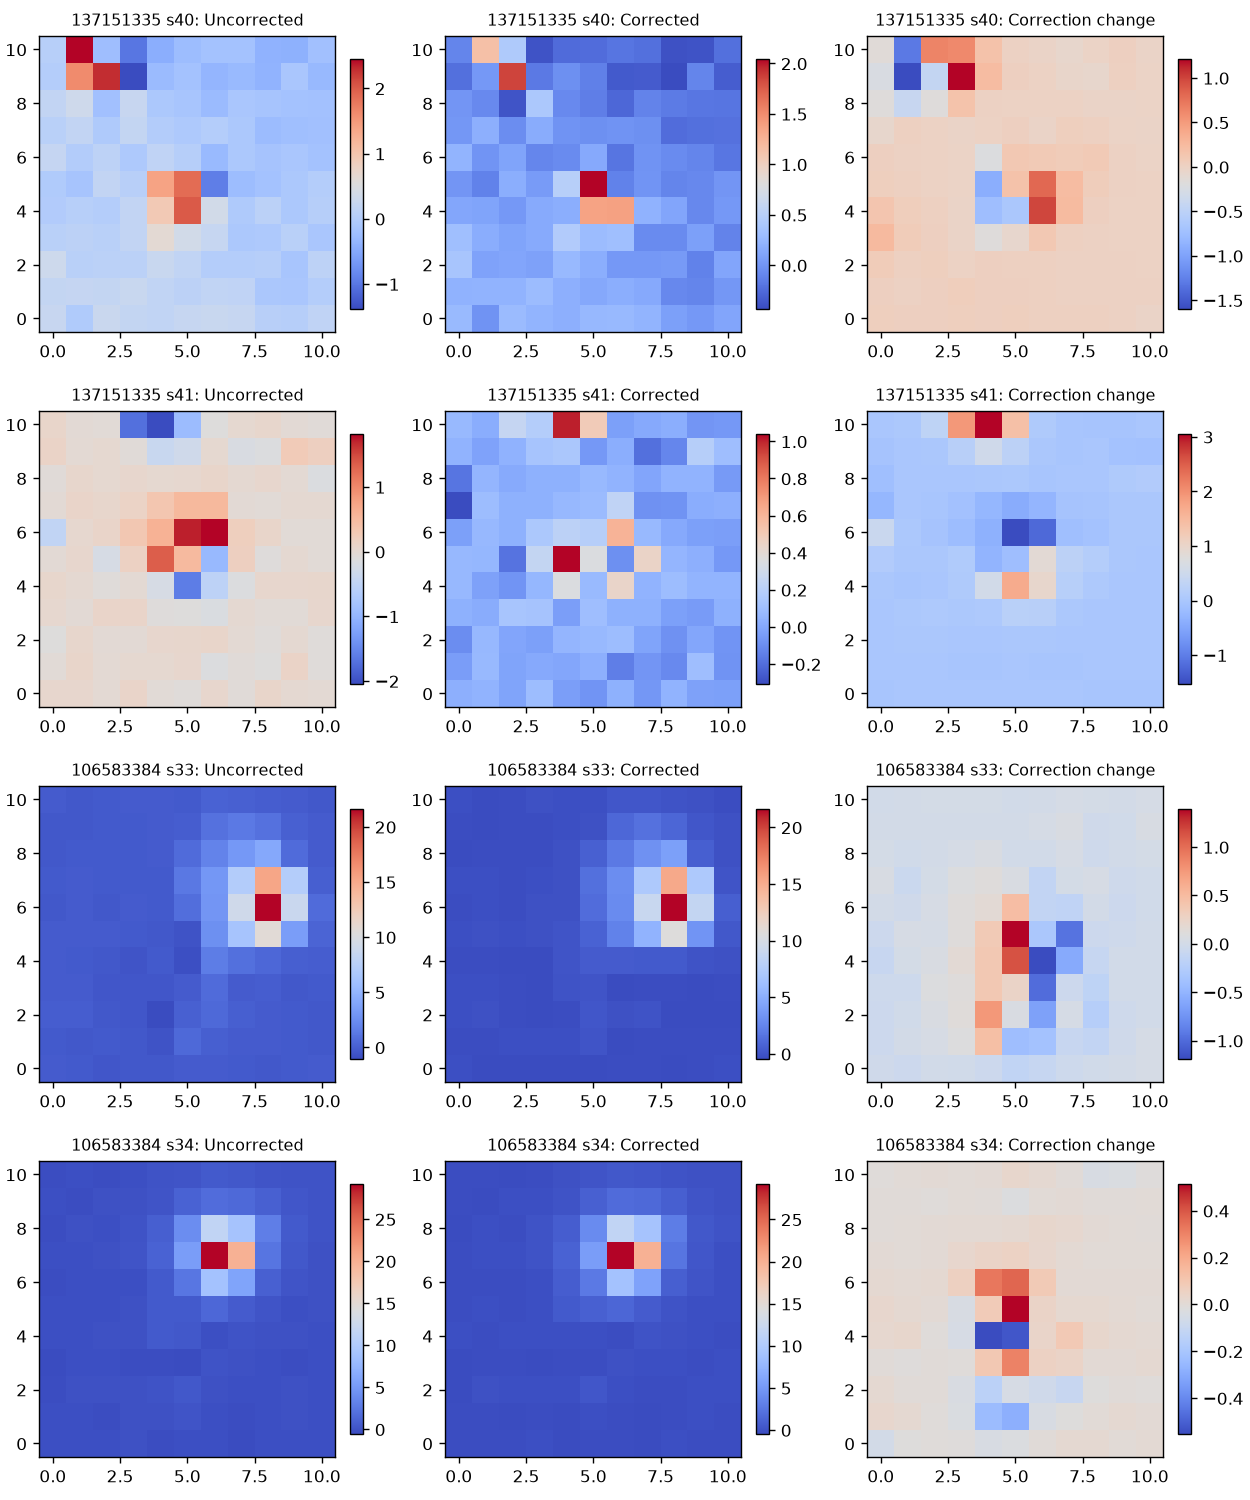
\includegraphics[width=\linewidth,height=0.72\textheight,keepaspectratio]{figures/controls-pointing.png}
\caption{Pointing-correction controls: three of four satisfy the frozen criterion. The Kepler-93 wrong-host case improves, but discrimination decreases in one contaminant sector. The complete gate therefore fails and the method is not applied to infer candidate hosts.}
\end{figure}
\begin{figure}[p]
\centering
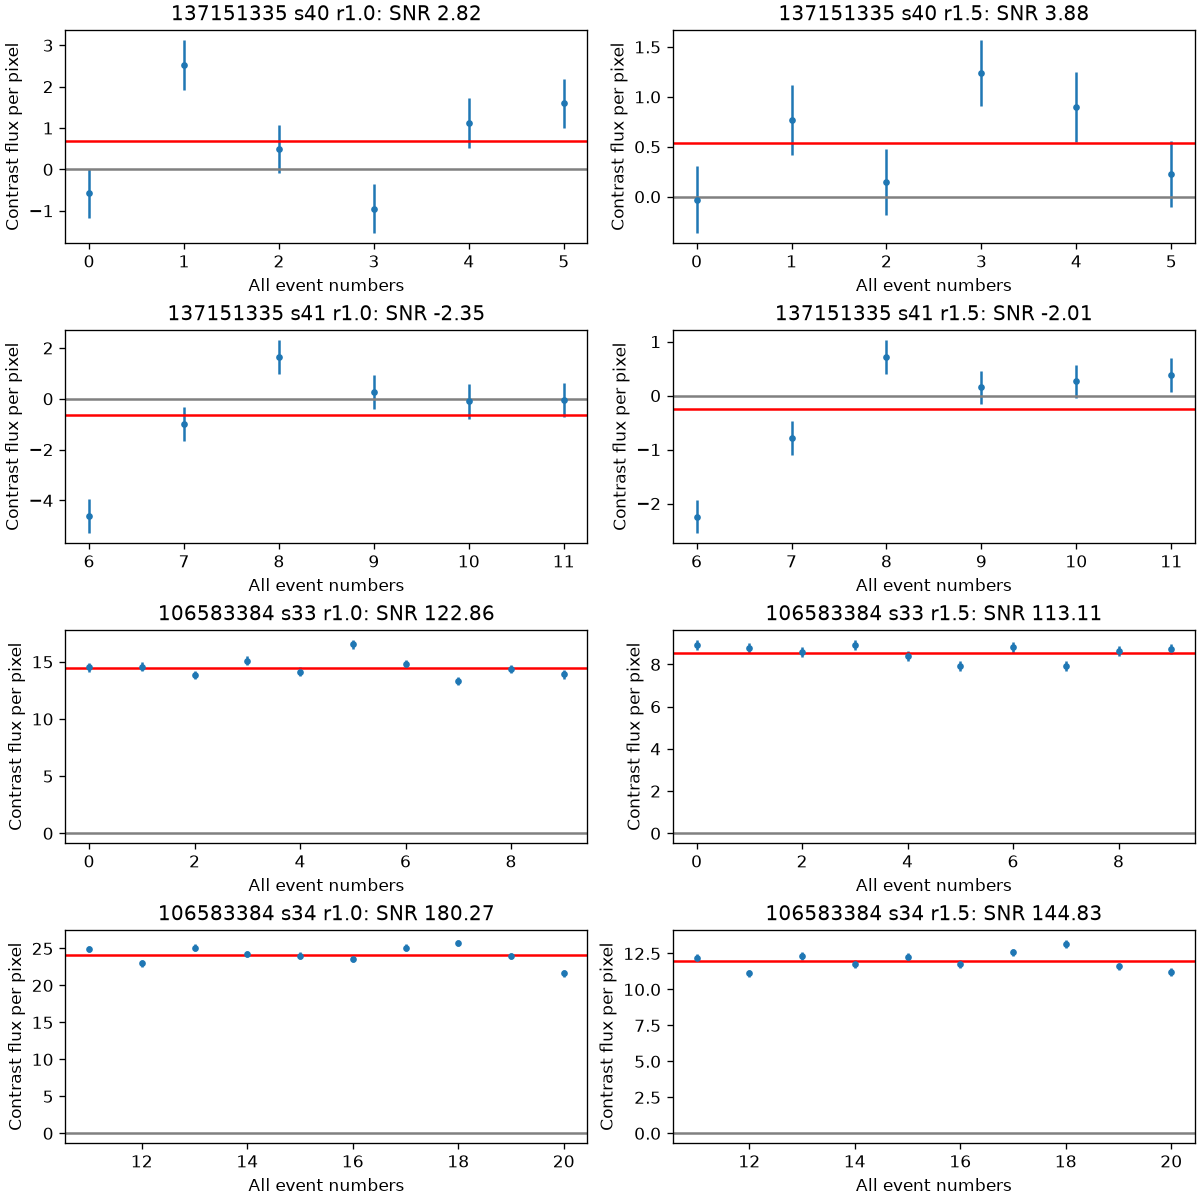
\includegraphics[width=\linewidth,height=0.72\textheight,keepaspectratio]{figures/controls-aperture.png}
\caption{Paired-aperture controls: five of eight sector/radius cases pass. Kepler-93 failures include a weak target measurement and wrong-region contrasts. The ordinate measures differential variable flux per exclusive pixel, not stellar fractional eclipse depth or calibrated throughput. The candidate-application gate fails.}
\end{figure}
\begin{figure}[p]
\centering
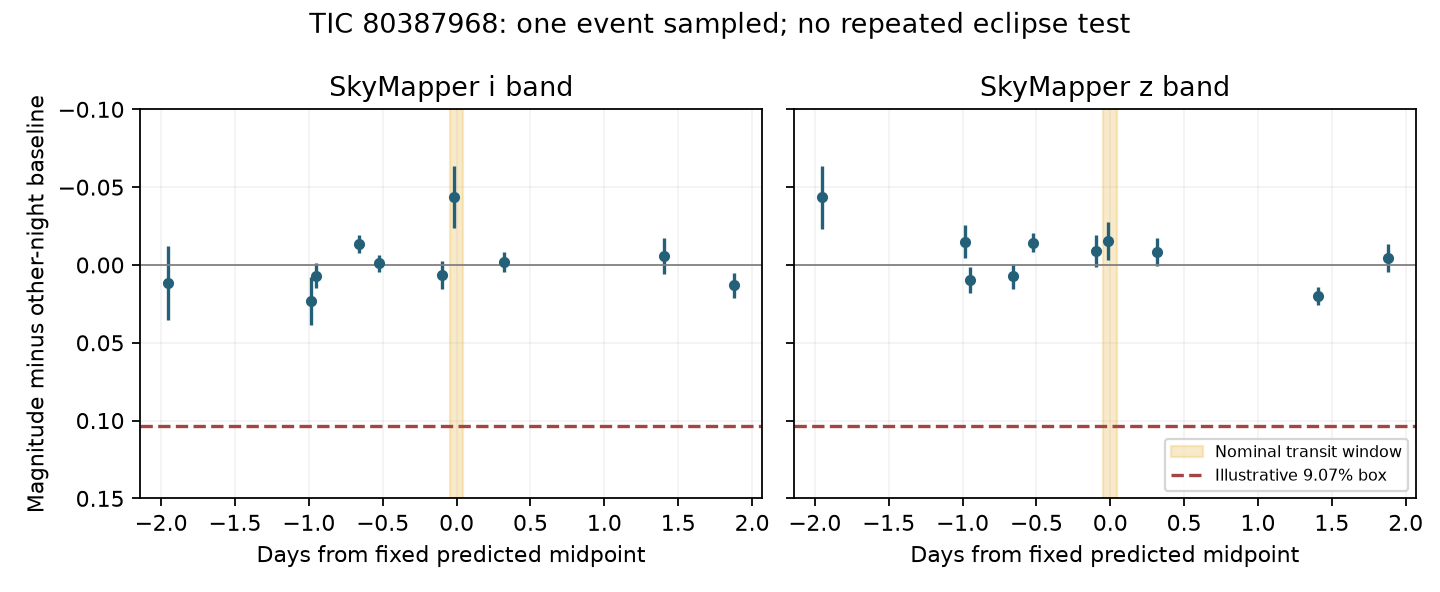
\includegraphics[width=\linewidth,height=0.72\textheight,keepaspectratio]{figures/803-resolved.png}
\caption{Resolved SkyMapper samples for neighbor TIC 80387968. Two measurements in different filters sample one predicted event without dimming, weakening a specified same-depth eclipse at those instants. The required two-event exclusion gate fails; sparse color-dependent samples do not clear the neighbor.}
\end{figure}
\begin{figure}[p]
\centering
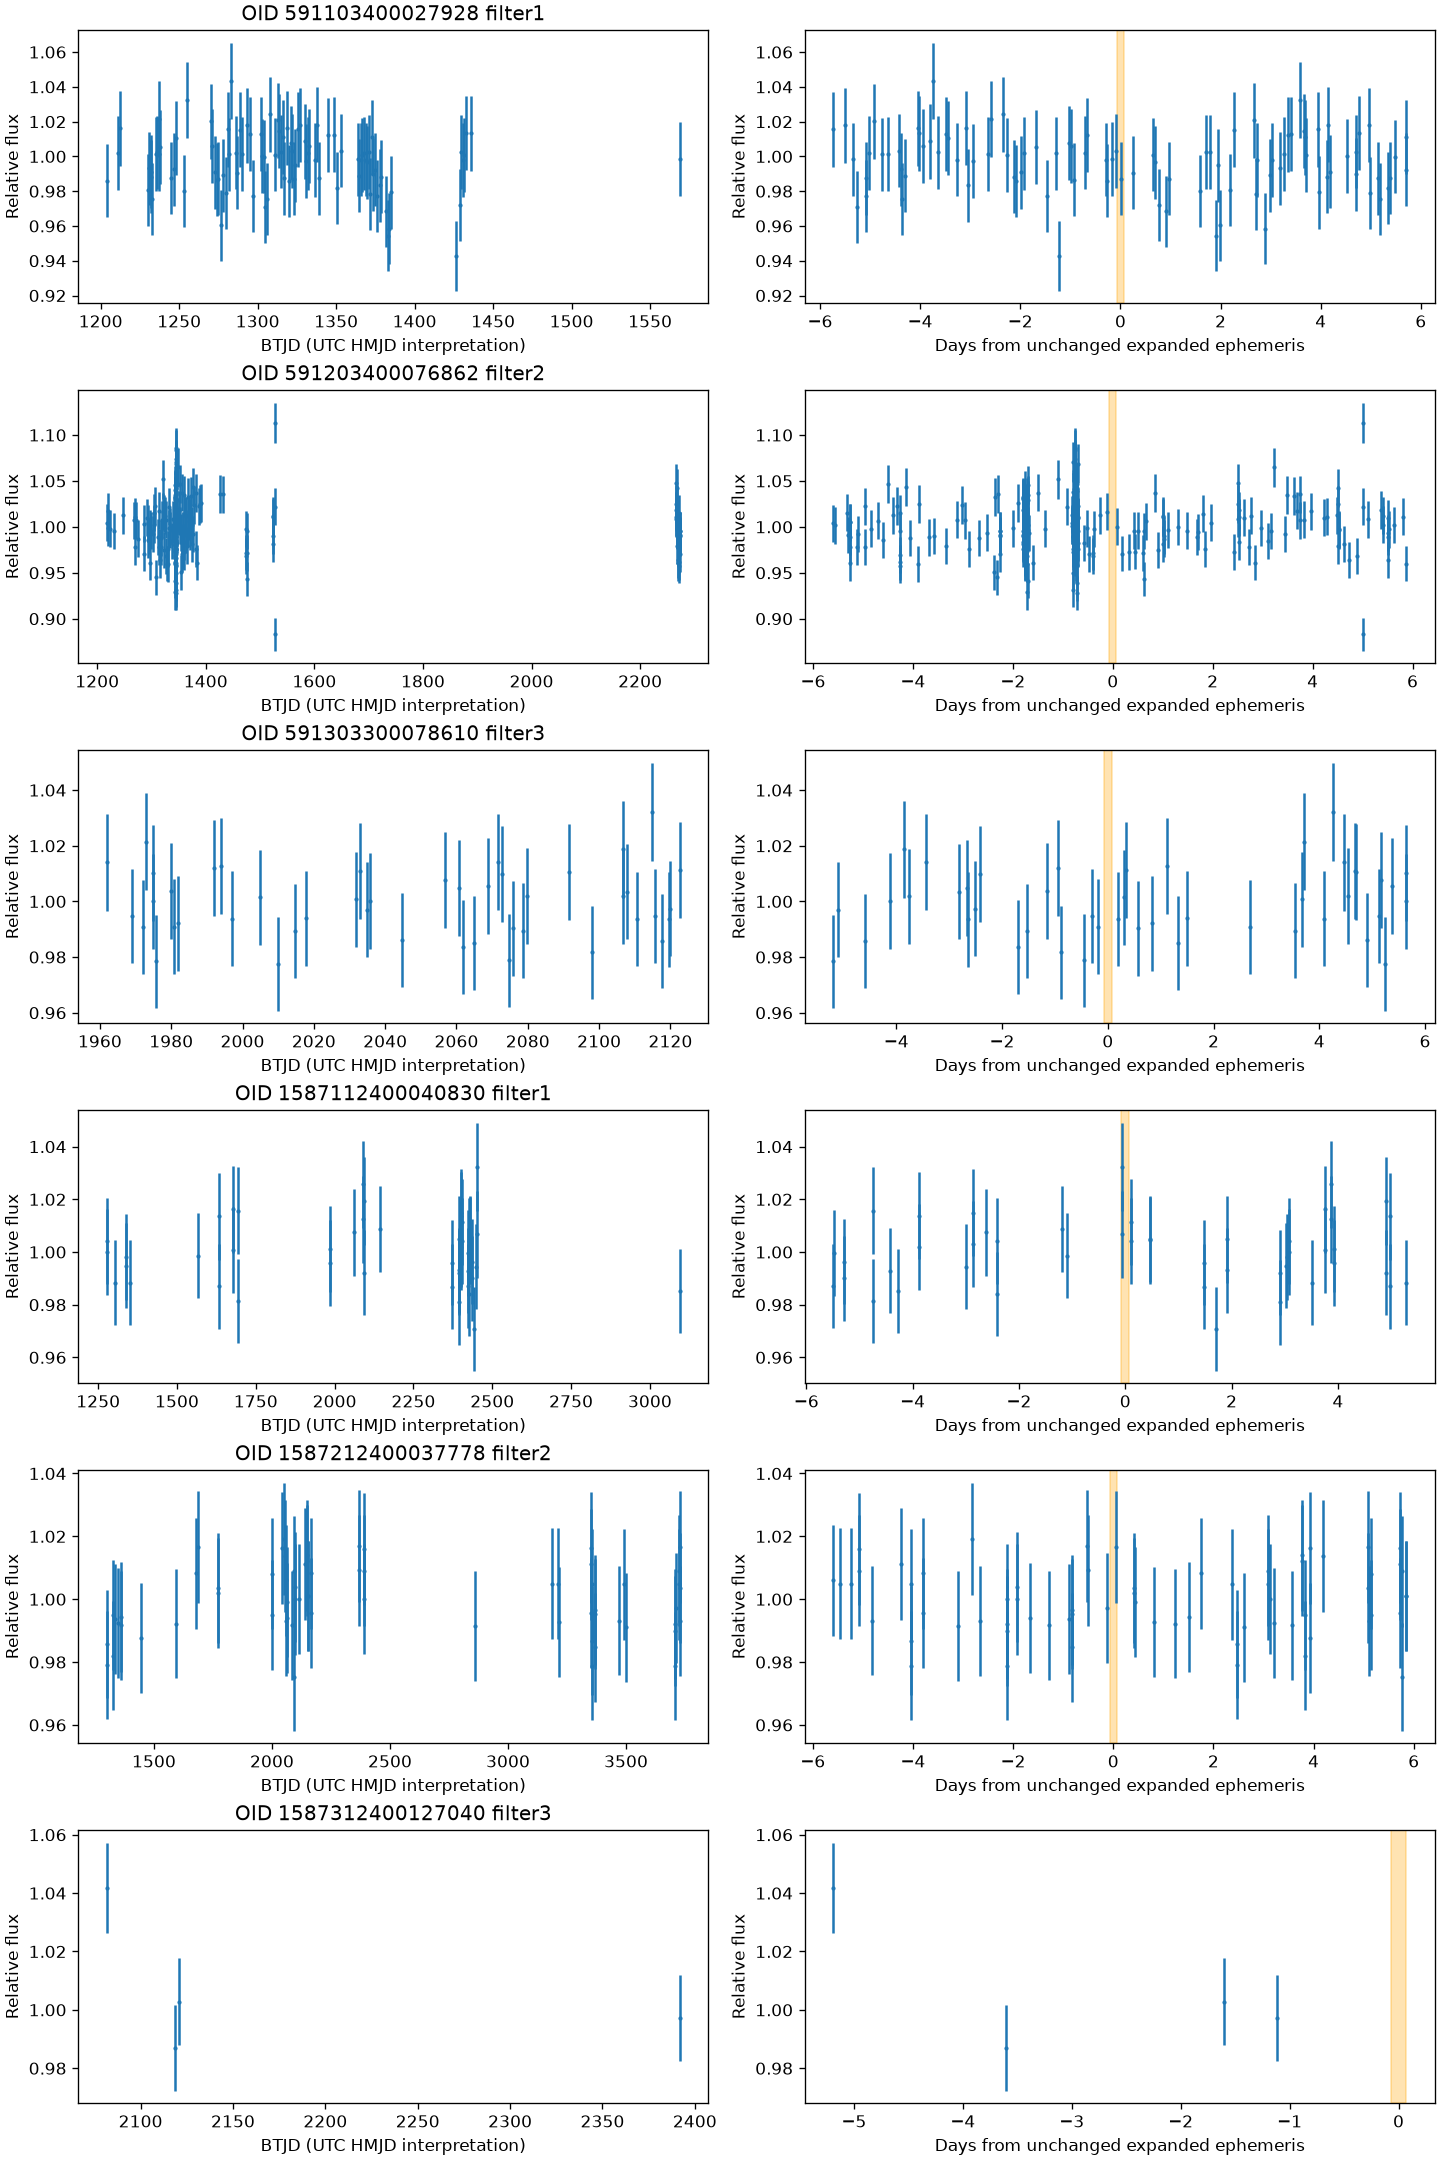
\includegraphics[width=\linewidth,height=0.72\textheight,keepaspectratio]{figures/402-resolved.png}
\caption{Resolved ZTF measurements for neighbor TIC 74037550 near TIC 402358350. Six streams contain 836 retrieved and 545 quality-selected points. All 72 clock/time-convention/stream-or-filter comparisons remain inconclusive; these plots provide neither a recovered eclipse nor a neighbor exclusion.}
\end{figure}
\begin{figure}[p]
\centering
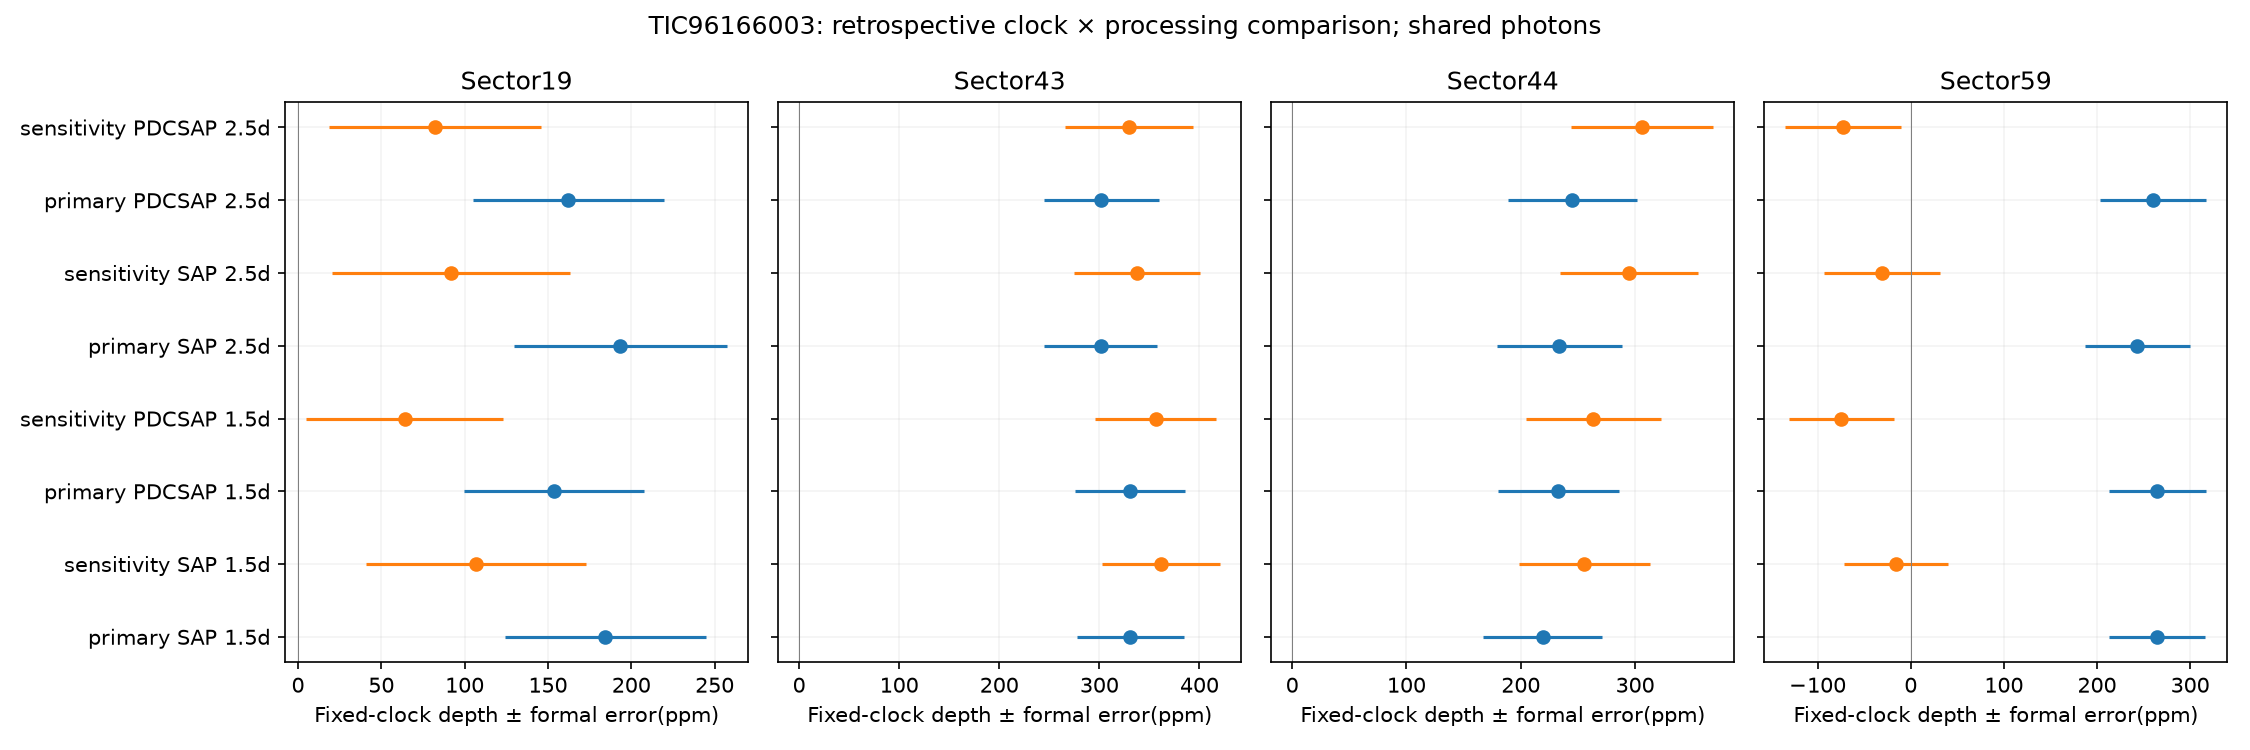
\includegraphics[width=\linewidth,height=0.72\textheight,keepaspectratio]{figures/961-clocks.png}
\caption{Crossed clock and processing comparison for TIC 96166003 sector 59. The expanded primary clock retains dimming across SAP/PDC and two detrending choices, whereas its alternative is negative or near zero. Shared-photon processing agreement does not identify the correct clock, and the original prediction timing remains inadequate.}
\end{figure}
\begin{figure}[p]
\centering
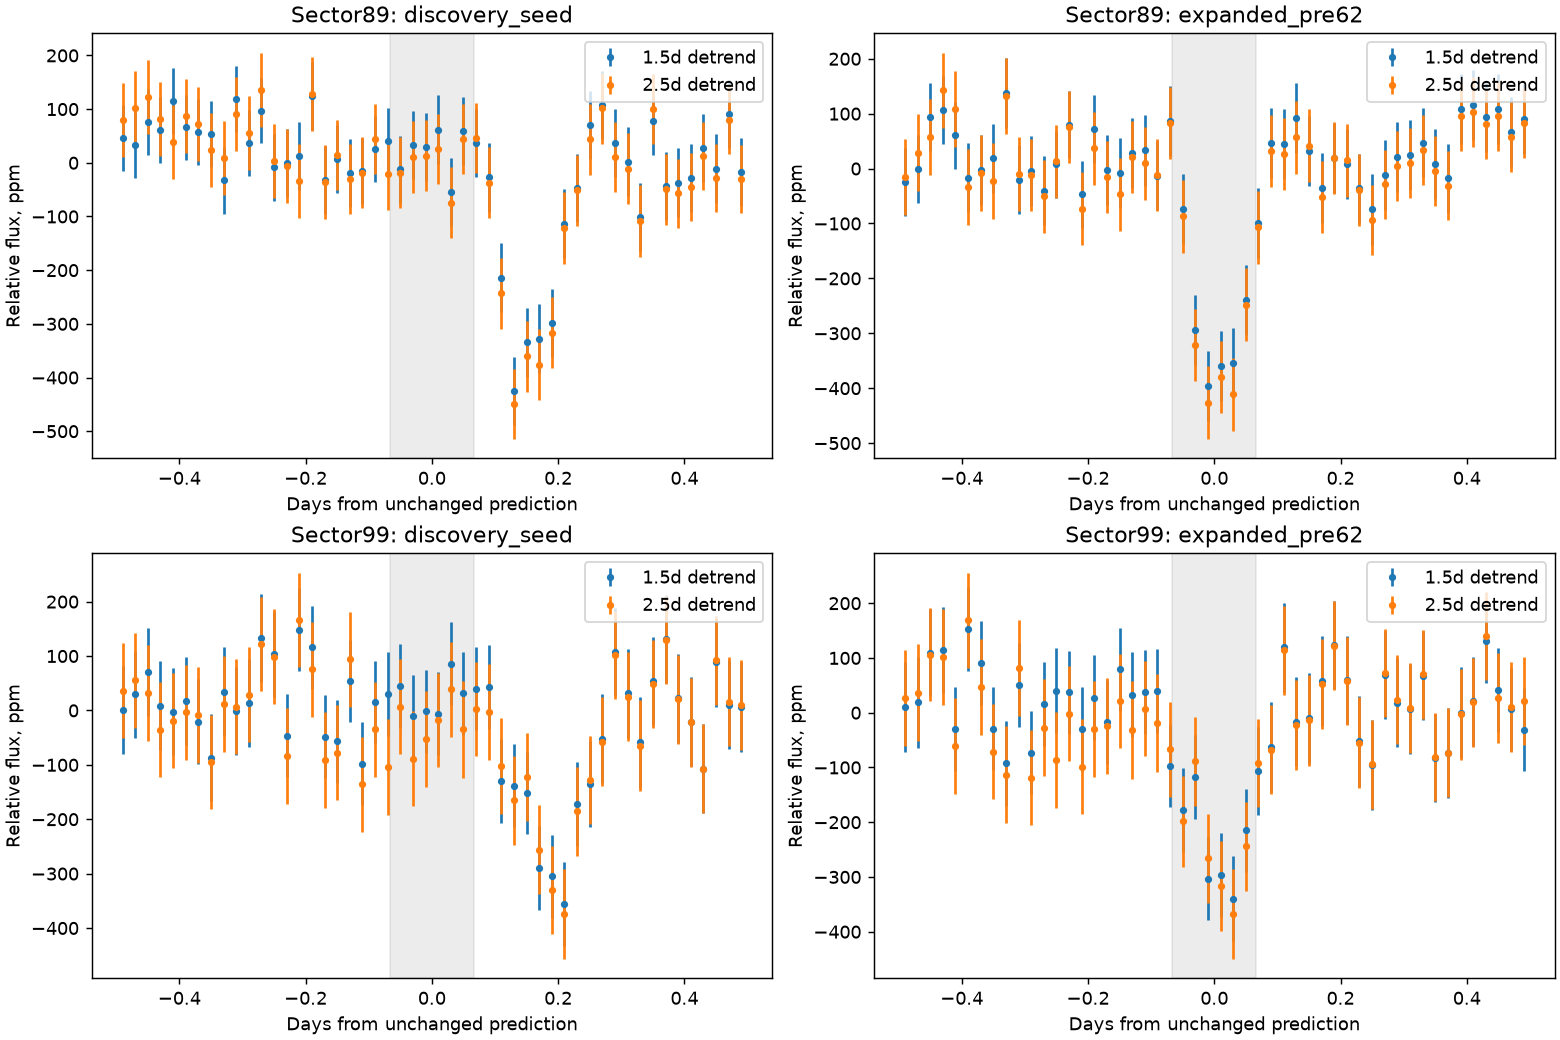
\includegraphics[width=\linewidth,height=0.72\textheight,keepaspectratio]{figures/554-new.png}
\caption{TIC 5546257 sectors 89 and 99 at the saved clock alternatives. Expanded-clock dips remain positive but fail the original timing gate; the coarse seed is unfavorable. Extraction and aperture differences limit physical depth comparisons. Neighbor Gaia variability strengthens contamination independently of these blended reductions.}
\end{figure}
\clearpage
